\documentclass[10pt,aspectratio=1610,compress,dvipsnames]{beamer}

\makeatletter
\def\input@path{{tex/}{chapters/}}
\makeatother

\usepackage{kotex}
\usetheme[
%%% option passed to the outer theme
%    progressstyle=fixedCircCnt,   % fixedCircCnt, movingCircCnt (moving is deault)
]{CodingTeal}

% If you want to change the colors of the various elements in the theme, edit and uncomment the following lines

% Change the bar colors:
%\setbeamercolor{CodingTeal}{fg=red!20,bg=red}

% Change the color of the structural elements:
%\setbeamercolor{structure}{fg=red}

% Change the frame title text color:
%\setbeamercolor{frametitle}{fg=blue}

% Change the normal text color background:
%\setbeamercolor{normal text}{fg=black,bg=gray!10}

%-------------------------------------------------------
% INCLUDE PACKAGES
%-------------------------------------------------------

%\usepackage[utf8]{inputenc}
%\usepackage[spanish,es-tabla]{babel}
%\usepackage[T1]{fontenc}
\usepackage{helvet}

%\usepackage[T1]{fontenc}
%\usepackage[utf8]{inputenc}
%\usepackage{newpxtext}
%\usepackage{newpxmath}

\usepackage[T1]{fontenc}
\usepackage[utf8]{inputenc}
\usepackage{textcomp}
\renewcommand{\ttdefault}{lmtt} % 
%-------------------------------------------------------
% DEFFINING AND REDEFINING COMMANDS
%-------------------------------------------------------
% colored hyperlinks
\newcommand{\chref}[2]{
	\href{#1}{{\usebeamercolor[bg]{CodingTeal} #2}}
}

\makeatletter
\def\blfootnote{\gdef\@thefnmark{}\@footnotetext}
\makeatother

%-------------------------------------------------------
% THE BODY OF THE PRESENTATION
%-------------------------------------------------------

\usepackage{listings} % For code highlighting with lstlisting

\usepackage{tikz}
\usepackage{pgfplots, pgfplotstable}
\pgfplotsset{compat=1.18}
\usetikzlibrary{positioning, shapes.geometric, arrows}
\usetikzlibrary{patterns} % Load the patterns library
\usetikzlibrary{positioning} % Load the positioning library
\usetikzlibrary{decorations.markings, arrows.meta}
\usetikzlibrary{decorations.pathmorphing}
\usetikzlibrary{bending, shadows.blur}
\usetikzlibrary{fit, calc, shapes}
\usetikzlibrary {mindmap}

\usepackage{multicol}
\renewcommand{\lstlistingname}{Code}
\usepackage{array}
\usepackage{booktabs}
\usepackage{adjustbox}
\usepackage{kotex}

\usepackage{pdfrender}
%-------------------------------------------------------
% INFORMATION IN THE TITLE PAGE
%-------------------------------------------------------

\title[Coding Theory] % [] is optional - is placed on the bottom of the sidebar on every slide
{ % is placed on the title page
		\textbf{\Huge Linear, Hamming, and Cyclic Codes} 
%	{\rmfamily\large by Almeida et al.}
%		\textbf{\fontsize{15.8}{16}\selectfont Verifying cryptographic implementations with Jasmin \& EasyCrypt}
}
\subtitle[Linear, Hamming, and Cyclic Codes]
{
		\text{\LARGE-- A Mathematician's Introduction --}
	%	\text{\color{gray}\small The Association for Computing Machinery,}\\
	%	\text{\color{gray}\small Conference on Computer and Communications Security}
}


\definecolor{cseteal}{HTML}{008C8C}
\definecolor{csedarkteal}{HTML}{003F46}
\author[Ji, Yong-hyeon]
{\texorpdfstring{   
		\vspace{.5cm}
%	\textpdfrender{
%%		TextRenderingMode=FillStroke,
%%		LineWidth=.05pt,
	%%		FillColor=cseteal,
%		TextRenderingMode=FillStrokeClip,
%		LineWidth=.5pt,
	%		FillColor=cseteal,
	%		StrokeColor=csedarkteal,
%	}{\textbf{\Large\selectfont Ji, Yong-hyeon}}\\
%	\color{cseteal}\textbf{\fontsize{14}{10}\selectfont Ji, Yong-hyeon} \\
	{\centering
		
\includegraphics[scale=1.5]{tikzs/jyh.pdf}
		}\\ [-.2cm]
		\color{black} \texttt{hacker3740@gmail.com}
}{Ji, Yong-hyeon}}

\institute[Enjoying Math]
{
	\vspace{.5cm}
	\textbf{\Large
		%\fontsize{11}{12}\selectfont 
		[기대수 3기 Colloquium]
%		Department of Information, Security, Cryptology and Mathematics
%Crypto \& Security Engineering Laboratory
	}\\
%	\fontsize{11}{12}\selectfont College of Science and Technology\\ \fontsize{11}{12}\selectfont Kookmin University\\
	\vspace{-0.5cm}
%	
\includegraphics[scale=0.2]{assets/branding/Ciencias-Quimicas.png} \\
	\vspace{1cm}
   	\textbf{\large\it 수학의 즐거움, Enjoying Math}\\
	\vspace{-1cm}
	
	%there must be an empty line above this line - otherwise some unwanted space is added between the university and the country (I do not know why;( )
}

\date{May 02, 2026}

\usepackage{tcolorbox}
\tcbset{colback=white, arc=5pt}

\definecolor{axiomcolor}{HTML}{00646A}
\definecolor{defcolor}{HTML}{007575}
\definecolor{procolor}{HTML}{00575E}
\definecolor{thmcolor}{HTML}{003F46}
\definecolor{lemcolor}{HTML}{006F73}
\definecolor{corcolor}{HTML}{00615F}
\definecolor{execolor}{HTML}{004F54}

% Define a new command for the custom tcolorbox
\newcommand{\axiombox}[2][]{%
	\begin{tcolorbox}[colframe=axiomcolor, title={\color{white}\bfseries #1}]
		#2
	\end{tcolorbox}
}

\newcommand{\defbox}[2][]{%
	\begin{tcolorbox}[colframe=defcolor, title={\color{white}\bfseries #1}]
		#2
	\end{tcolorbox}
}

\newcommand{\lembox}[2][]{%
	\begin{tcolorbox}[colframe=lemcolor, title={\color{white}\bfseries #1}]
		#2
	\end{tcolorbox}
}

\newcommand{\probox}[2][]{%
	\begin{tcolorbox}[colframe=procolor, title={\color{white}\bfseries #1}]
		#2
	\end{tcolorbox}
}

\newcommand{\thmbox}[2][]{%
	\begin{tcolorbox}[colframe=thmcolor, title={\color{white}\bfseries #1}]
		#2
	\end{tcolorbox}
}

\newcommand{\corbox}[2][]{%
	\begin{tcolorbox}[colframe=corcolor, title={\color{white}\bfseries #1}]
		#2
	\end{tcolorbox}
}

\input{tex/listing}
% Pseudo-code
\usepackage[linesnumbered,ruled]{algorithm2e}
\usepackage{algorithmicx}
\usepackage{algpseudocode}
%\usepackage{setspace}
\SetKwComment{Comment}{/* }{ */}
\SetKwProg{Fn}{Function}{:}{end}
\SetKwProg{Procedure}{Procedure}{:}{end}
\SetKw{End}{end}
\SetKw{DownTo}{downto}
\newcommand{\F}{\mathbb{F}}
\newcommand{\Z}{\mathbb{Z}}
\newcommand{\N}{\mathbb{N}}
\newcommand{\R}{\mathbb{R}}

\newcommand{\gen}[1]{\langle #1\rangle}
\newcommand{\ideal}[1]{\langle #1\rangle}
\newcommand{\code}{\mathcal{C}}
\newcommand{\set}[1]{\left\{#1\right\}}
\newcommand{\wt}{\operatorname{wt}}
\newcommand{\rank}{\operatorname{rank}}
\newcommand{\Span}{\operatorname{span}}
\newcommand{\Aut}{\operatorname{Aut}}
\newcommand{\supp}{\operatorname{supp}}
\newcommand{\ol}[1]{\overline{#1}}

\newcommand{\nkcode}[3]{[#1,#2]_{#3}}
\newcommand{\nkdcode}[4]{[#1,#2,#3]_{#4}}

\newcommand{\fullfunction}[5]{%
  \begin{array}{r@{\;}c@{\;}l}
    #1\colon #2 &\longrightarrow& #3 \\[2pt]
    #4 &\longmapsto& #5
  \end{array}
}


\usepackage{soul}
\usepackage{colortbl}
\usepackage{booktabs}
\usetikzlibrary{tikzmark}
\renewcommand{\vec}[1]{\mathbf{#1}}

\begin{document}

%-------------------------------------------------------
% TITLE PAGE
%-------------------------------------------------------
\begin{frame}[plain,noframenumbering]
  \titlepage
\end{frame}

%-------------------------------------------------------
% TABLE OF CONTENTS
%-------------------------------------------------------
\section*{Contents}
\begin{frame}{\textbf{Contents}}
  \tableofcontents
\end{frame}

%-------------------------------------------------------
% I. INTRODUCTION
%-------------------------------------------------------
\section{I. Introduction}
%=======================================================
% CHAPTER 0: INTRODUCTION
%=======================================================

%--- Section Title Frame ---
\begin{frame}[plain]
  \begin{center}\bfseries\centering
    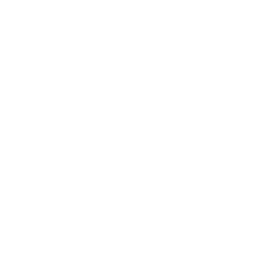
\includegraphics[scale=1]{assets/branding/opa0}
    \vspace{-5.75cm}\\
    {\adjustbox{scale=2.5}{\color{TealDarkCyan}\;I.\;Introduction}}
    \bigskip\bigskip
    {\ }\vspace{4cm}\\
    \bigskip
  \end{center}
\end{frame}

%--- Slide: The Communication Problem ---
\begin{frame}{\textbf{I. Introduction}}{The Communication Problem}
\begin{center}
\begin{tikzpicture}[
  cbox/.style   = {draw, thick, rounded corners=4pt, minimum height=.85cm,
                   minimum width=1.8cm, align=center},
  arr/.style    = {-Stealth, thick, color=TealDarkCyan},
  noise/.style  = {-Stealth, thick, color=AccentCyan!80!black},
  lbl/.style    = {font=\small}
]
  \node[cbox, fill=TealDarkCyan!15] (src) {\small Source\\[-2pt]$\mathbf{m}$};
  \node[cbox, fill=TealDarkCyan!25, right=1.1cm of src]  (enc) {\small Encoder};
  \node[cbox, fill=AccentCyan!18,    right=1.1cm of enc]  (ch)  {\small Noisy\\[-2pt]\small Channel};
  \node[cbox, fill=TealDarkCyan!25, right=1.1cm of ch]   (dec) {\small Decoder};
  \node[cbox, fill=TealDarkCyan!15, right=1.1cm of dec]  (dst) {\small Receiver\\[-2pt]$\hat{\mathbf{m}}$};
  \node[above=.55cm of ch, AccentCyan!80!black]    (err) {\small $\mathbf{e}$\; (noise)};

  \draw[arr] (src) -- (enc) node[midway,above,lbl]{$\mathbf{m}$};
  \draw[arr] (enc) -- (ch)  node[midway,above,lbl]{$\mathbf{c}$};
  \draw[arr] (ch)  -- (dec) node[midway,above,lbl]{$\mathbf{v}=\mathbf{c}+\mathbf{e}$};
  \draw[arr] (dec) -- (dst) node[midway,above,lbl]{$\hat{\mathbf{m}}$};
  \draw[noise] (err) -- (ch);
\end{tikzpicture}
\end{center}
\bigskip
\begin{columns}[T,onlytextwidth]
  \begin{column}{.48\textwidth}
    \textbf{Setup}
    \begin{itemize}\small
      \item Message $\mathbf{m}\in\F_q^k$
      \item Encoder adds redundancy: $\mathbf{m}\mapsto\mathbf{c}\in\F_q^n$,\; $n>k$
      \item Channel corrupts: $\mathbf{v}=\mathbf{c}+\mathbf{e}$
    \end{itemize}
  \end{column}
  \begin{column}{.48\textwidth}
    \textbf{Goal}
    \begin{itemize}\small
      \item Recover $\hat{\mathbf{m}}=\mathbf{m}$ even when $\mathbf{e}\neq\mathbf{0}$
      \item Keep rate $R = k/n$ as large as possible
    \end{itemize}
  \end{column}
\end{columns}
\end{frame}

%--- Slide: Shannon's Theorem ---
\begin{frame}{\textbf{I. Introduction}}{Shannon's Channel Coding Theorem (1948)}

\defbox[Shannon's Channel Coding Theorem]{
For any discrete memoryless channel with capacity $C$ and any rate $R<C$, there exists a sequence of codes of rate $\to R$ whose block error probability $\to 0$.
}

\bigskip
\begin{columns}[T,onlytextwidth]
  \begin{column}{.48\textwidth}
    \textcolor{TealDarkCyan}{\textbf{What it guarantees}}
    \begin{itemize}\small
      \item Reliable communication \emph{is} possible below capacity
      \item Error probability can be made arbitrarily small
    \end{itemize}
  \end{column}
  \begin{column}{.48\textwidth}
    \textcolor{AccentCyan!80!black}{\textbf{What it does not provide}}
    \begin{itemize}\small
      \item \emph{How} to construct such codes explicitly
      \item \emph{How} to decode efficiently
    \end{itemize}
  \end{column}
\end{columns}

\bigskip
\begin{alertblock}{The Central Challenge of Coding Theory}
\centering
Construct \textbf{explicit algebraic codes} that are both \textbf{efficient} (high rate) and \textbf{powerful} (correct many errors).
\end{alertblock}
\end{frame}

%--- Slide: Roadmap ---
\begin{frame}{\textbf{I. Introduction}}{Roadmap}

\begin{columns}[T,onlytextwidth]
  \begin{column}{.48\textwidth}
    \defbox[II.\;Linear Codes]{
    \small Structure via \textbf{linear algebra}
    \begin{itemize}
      \item[$\bullet$] Subspaces of $\F_q^n$
      \item[$\bullet$] Generator $G$, parity-check $H$
      \item[$\bullet$] Hamming distance \& error correction
    \end{itemize}
    }
    \medskip
	    \defbox[III.\;Hamming Codes]{
	    \small Perfect codes via \textbf{projective geometry}
	    \begin{itemize}
	      \item[$\bullet$] Parity checks from projective points
	      \item[$\bullet$] Syndrome decoding as geometry
	      \item[$\bullet$] Perfect single-error correction
	    \end{itemize}
	    }
	  \end{column}
	  \begin{column}{.48\textwidth}
	    \defbox[IV.\;Cyclic Codes]{
	    \small
	    Structure via \textbf{polynomial rings}
	    \begin{itemize}
	      \item[$\bullet$] Quotient $\F_q[X]/(X^n-1)$
	      \item[$\bullet$] Ideals and generator polynomials
	      \item[$\bullet$] BCH design and cyclic Hamming codes
	    \end{itemize}
	    }
	    \bigskip
	    \begin{block}{Key Observation}
	    \small Coding theory is a meeting point of \textbf{linear algebra}, \textbf{finite geometry}, and \textbf{polynomial algebra}.
	    \end{block}
  \end{column}
\end{columns}
\end{frame}


%-------------------------------------------------------
% II. LINEAR CODES
%-------------------------------------------------------
\section{II. Linear Codes}
%=======================================================
% CHAPTER 1: LINEAR CODES
%=======================================================

\begin{frame}[plain]
  \begin{center}\bfseries\centering
    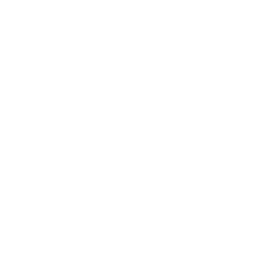
\includegraphics[scale=1]{assets/branding/opa0}
    \vspace{-5.75cm}\\
    {\adjustbox{scale=2.15}{\color{TealDarkCyan}\;II.\;Linear Codes}}
    \bigskip\bigskip
    {\ }\vspace{4cm}\\
    \bigskip
  \end{center}
\end{frame}

\begin{frame}{\textbf{II. Linear Codes}}{The ambient space}
\small
\defbox[Hamming space]{
Fix a finite field $\F_q$. The set $\F_q^n$ is simultaneously a vector space and a metric space with
\[
  d(x,y)=\#\{i:x_i\ne y_i\}.
\]
}
\begin{itemize}
  \item The metric is translation invariant: $d(x+z,y+z)=d(x,y)$.
  \item The spheres are combinatorial objects:
  \[
    |B_t(0)|=\sum_{i=0}^t \binom{n}{i}(q-1)^i.
  \]
  \item Coding theory asks for large subsets with large mutual distance.
\end{itemize}
\end{frame}

\begin{frame}{\textbf{II. Linear Codes}}{Codes as metric subsets}
\small
\defbox[Code]{
A code of length $n$ over $\F_q$ is a subset $\code\subseteq \F_q^n$. Its minimum distance is
\[
  d(\code)=\min\{d(x,y):x,y\in\code,\ x\ne y\}.
\]
}
\begin{block}{Mathematician's viewpoint}
The fundamental problem is an extremal problem in a finite metric space:
\[
  A_q(n,d)=\max\{|\code|:\code\subseteq\F_q^n,\ d(\code)\ge d\}.
\]
\end{block}
\end{frame}

\begin{frame}{\textbf{II. Linear Codes}}{Linearity}
\small
\defbox[Linear code]{
A linear $[n,k,d]_q$ code is a $k$-dimensional subspace
\[
  \code\le \F_q^n
\]
with minimum distance $d$.
}
\begin{itemize}
  \item The cardinality is forced: $|\code|=q^k$.
  \item The rate is $R=k/n$.
  \item Since $\code$ is a group under addition,
  \[
    d(\code)=\min\{\wt(c):0\ne c\in\code\}.
  \]
\end{itemize}
\end{frame}

\begin{frame}{\textbf{II. Linear Codes}}{Weight}
\small
\defbox[Hamming weight]{
For $x=(x_1,\ldots,x_n)\in\F_q^n$,
\[
  \wt(x)=|\supp(x)|,\qquad \supp(x)=\{i:x_i\ne0\}.
\]
}
\begin{block}{Lemma}
For a linear code $\code$,
\[
  d(\code)=\min_{0\ne c\in\code}\wt(c).
\]
\end{block}
\textbf{Proof.} If $x,y\in\code$, then $x-y\in\code$ and $d(x,y)=\wt(x-y)$.
\end{frame}

\begin{frame}{\textbf{II. Linear Codes}}{Generator matrices}
\small
\defbox[Generator matrix]{
A generator matrix for an $[n,k]_q$ code is a matrix $G\in\F_q^{k\times n}$ whose rows form a basis of $\code$.
Encoding is the linear map
\[
  \F_q^k\longrightarrow \F_q^n,\qquad m\longmapsto mG.
\]
}
\begin{itemize}
  \item The code is the row space of $G$.
  \item Different bases give different generator matrices for the same code.
  \item Replacing $G$ by $UG$, $U\in\operatorname{GL}_k(\F_q)$, changes coordinates on messages only.
\end{itemize}
\end{frame}

\begin{frame}{\textbf{II. Linear Codes}}{Equivalence of descriptions}
\small
\thmbox[Row-space equivalence]{
Two full-rank matrices $G,G'\in\F_q^{k\times n}$ generate the same code if and only if
\[
  G'=UG
\]
for some $U\in\operatorname{GL}_k(\F_q)$.
}
\begin{itemize}
  \item This is just change of basis in the subspace $\code$.
  \item The code is the invariant object; the matrix is a coordinate choice.
  \item Many computational algorithms are Gaussian elimination on this statement.
\end{itemize}
\end{frame}

\begin{frame}{\textbf{II. Linear Codes}}{Systematic form}
\small
\defbox[Systematic generator matrix]{
After permuting coordinates, many generator matrices can be written
\[
  G=[I_k\mid P].
\]
}
\begin{itemize}
  \item The message appears visibly in the first $k$ coordinates.
  \item The remaining $n-k$ coordinates are parity symbols.
  \item Systematic form is convenient, but it is not an intrinsic property of the code.
\end{itemize}
\begin{block}{Caution}
Coordinate permutations preserve distance, but they change the visible positions of message and parity symbols.
\end{block}
\end{frame}

\begin{frame}{\textbf{II. Linear Codes}}{Parity-check matrices}
\small
\defbox[Parity-check matrix]{
A parity-check matrix is a matrix $H\in\F_q^{(n-k)\times n}$ such that
\[
  \code=\ker(H)=\{c\in\F_q^n:Hc^T=0\}.
\]
}
\begin{itemize}
  \item If $G$ generates $\code$, then $GH^T=0$.
  \item The rows of $H$ generate the dual code $\code^\perp$.
  \item The equation $Hc^T=0$ is a system of homogeneous parity constraints.
\end{itemize}
\end{frame}

\begin{frame}{\textbf{II. Linear Codes}}{Duality}
\small
\defbox[Dual code]{
The dual of $\code\le\F_q^n$ is
\[
  \code^\perp=\{y\in\F_q^n:\langle x,y\rangle=0\text{ for all }x\in\code\}.
\]
}
\begin{block}{Dimension identity}
\[
  \dim\code+\dim\code^\perp=n.
\]
\end{block}
\begin{itemize}
  \item A parity-check matrix for $\code$ is a generator matrix for $\code^\perp$.
  \item Duality exchanges constraints and codewords.
\end{itemize}
\end{frame}

\begin{frame}{\textbf{II. Linear Codes}}{Distance from checks}
\small
\thmbox[Column criterion]{
Let $H$ be a parity-check matrix of $\code$. Then $d(\code)$ is the least number of columns of $H$ that are linearly dependent.
}
\begin{proof}
A vector $c$ of weight $s$ satisfies $Hc^T=0$ exactly when a linear combination of the $s$ corresponding columns is zero.
\end{proof}
\begin{itemize}
  \item No zero column means $d\ge2$.
  \item No proportional columns means $d\ge3$.
  \item This criterion is the entrance to Hamming codes.
\end{itemize}
\end{frame}

\begin{frame}{\textbf{II. Linear Codes}}{Syndromes}
\small
\defbox[Syndrome]{
For a received word $v=c+e$, define
\[
  s(v)=Hv^T.
\]
Since $Hc^T=0$, one has
\[
  s(v)=He^T.
\]
}
\begin{itemize}
  \item The syndrome depends only on the error coset.
  \item $s(v)=0$ if and only if $v\in\code$.
  \item Decoding is the problem of choosing a likely error in each coset.
\end{itemize}
\end{frame}

\begin{frame}{\textbf{II. Linear Codes}}{Cosets}
\small
\defbox[Coset decomposition]{
The ambient space is a disjoint union of cosets:
\[
  \F_q^n=\coprod_{a\in A}(a+\code),
\]
where $|A|=q^{n-k}$.
}
\begin{itemize}
  \item All words in the same coset have the same syndrome.
  \item Syndromes parameterize cosets when $H$ has full rank.
  \item Decoding assigns to each coset a chosen representative of small weight.
\end{itemize}
\end{frame}

\begin{frame}{\textbf{II. Linear Codes}}{Standard arrays}
\small
\defbox[Coset leader]{
A coset leader is an element of least Hamming weight in a coset $a+\code$.
}
\begin{itemize}
  \item The standard array lists cosets by their leaders.
  \item Nearest-neighbor decoding subtracts the coset leader.
  \item The method is conceptually clean but exponential in $n-k$.
\end{itemize}
\begin{block}{Principle}
Good algebraic families replace the standard array by structure.
\end{block}
\end{frame}

\begin{frame}{\textbf{II. Linear Codes}}{Correction and detection}
\small
\thmbox[Distance theorem]{
A code of minimum distance $d$ detects every error of weight at most $d-1$ and corrects every error of weight at most
\[
  t=\left\lfloor\frac{d-1}{2}\right\rfloor.
\]
}
\begin{itemize}
  \item Detection: no nonzero error of weight $<d$ is a codeword.
  \item Correction: balls of radius $t$ around distinct codewords are disjoint.
\end{itemize}
\end{frame}

\begin{frame}{\textbf{II. Linear Codes}}{Packing}
\small
\thmbox[Hamming bound]{
If $\code$ is an $[n,k,d]_q$ code and $t=\lfloor(d-1)/2\rfloor$, then
\[
  q^k\sum_{i=0}^t \binom{n}{i}(q-1)^i\le q^n.
\]
}
\begin{proof}
The balls of radius $t$ around codewords are disjoint subsets of $\F_q^n$.
\end{proof}
\begin{block}{Perfect code}
Equality means the radius-$t$ balls tile the whole Hamming space.
\end{block}
\end{frame}

\begin{frame}{\textbf{II. Linear Codes}}{Singleton bound}
\small
\thmbox[Singleton bound]{
Every $[n,k,d]_q$ code satisfies
\[
  d\le n-k+1.
\]
}
\begin{proof}
Delete $d-1$ coordinates. Distinct codewords must remain distinct, so $q^k\le q^{n-d+1}$.
\end{proof}
\begin{itemize}
  \item Codes meeting the bound are called MDS codes.
  \item Reed--Solomon codes are the standard nonbinary MDS examples.
\end{itemize}
\end{frame}

\begin{frame}{\textbf{II. Linear Codes}}{Gilbert--Varshamov idea}
\small
\thmbox[Existence principle]{
There exist linear codes whose parameters are good because a greedy construction cannot cover the whole space too early.
}
\[
  q^k\sum_{i=0}^{d-2}\binom{n-1}{i}(q-1)^i < q^n
  \quad\Rightarrow\quad
  \text{an }[n,k,d]_q\text{ code exists.}
\]
\begin{itemize}
  \item This is not a construction one wants to implement.
  \item It proves that the asymptotic landscape is nontrivial.
  \item Algebraic families try to approach such existence bounds explicitly.
\end{itemize}
\end{frame}

\begin{frame}{\textbf{II. Linear Codes}}{Griesmer bound}
\small
\thmbox[Griesmer bound]{
For a linear $[n,k,d]_q$ code,
\[
  n\ge \sum_{i=0}^{k-1}\left\lceil \frac{d}{q^i}\right\rceil.
\]
}
\begin{itemize}
  \item This is stronger than Singleton in many small-parameter cases.
  \item It comes from repeatedly puncturing on the support of a minimum word.
  \item It is a linear-code bound: linearity is essential.
\end{itemize}
\end{frame}

\begin{frame}{\textbf{II. Linear Codes}}{Puncturing}
\small
\defbox[Puncturing]{
Puncturing a code at coordinate $i$ means deleting the $i$-th coordinate from every word.
}
\begin{itemize}
  \item Length decreases by one.
  \item Dimension usually stays the same, but can drop.
  \item Minimum distance can decrease by at most one.
\end{itemize}
\begin{block}{Use}
Puncturing is the basic operation for inductive arguments on code parameters.
\end{block}
\end{frame}

\begin{frame}{\textbf{II. Linear Codes}}{Shortening}
\small
\defbox[Shortening]{
Shortening at coordinate $i$ means first selecting codewords with $c_i=0$, then puncturing at $i$.
}
\begin{itemize}
  \item Length decreases by one.
  \item Dimension can decrease by one.
  \item Minimum distance does not decrease.
\end{itemize}
\begin{block}{Duality}
Puncturing and shortening are dual operations:
\[
  (\text{puncture } \code)^\perp=\text{shorten }(\code^\perp).
\]
\end{block}
\end{frame}

\begin{frame}{\textbf{II. Linear Codes}}{Weight enumerators}
\small
\defbox[Weight enumerator]{
The weight enumerator is
\[
  W_\code(X,Y)=\sum_{c\in\code}X^{n-\wt(c)}Y^{\wt(c)}.
\]
}
\begin{itemize}
  \item It records the distribution of weights.
  \item The minimum distance is the first nonzero exponent of $Y$ after the constant term.
  \item It is a coarser invariant than the code but a powerful one.
\end{itemize}
\end{frame}

\begin{frame}{\textbf{II. Linear Codes}}{MacWilliams identity}
\small
\thmbox[MacWilliams identity]{
For a linear $[n,k]_q$ code,
\[
  W_{\code^\perp}(X,Y)=\frac{1}{|\code|}W_\code(X+(q-1)Y,X-Y).
\]
}
\begin{itemize}
  \item The identity is a finite Fourier transform.
  \item It turns the weight distribution of $\code$ into that of $\code^\perp$.
  \item It is one of the central reasons duality is computationally useful.
\end{itemize}
\end{frame}

\begin{frame}{\textbf{II. Linear Codes}}{Self-orthogonality}
\small
\defbox[Self-orthogonal and self-dual]{
A code is self-orthogonal if $\code\subseteq\code^\perp$ and self-dual if $\code=\code^\perp$.
}
\begin{itemize}
  \item Self-dual binary codes have dimension $n/2$.
  \item Doubly-even self-dual codes have all weights divisible by $4$.
  \item Such codes connect coding theory to lattices and modular forms.
\end{itemize}
\end{frame}

\begin{frame}{\textbf{II. Linear Codes}}{Equivalent codes}
\small
\defbox[Monomial equivalence]{
Two $q$-ary linear codes are equivalent if one is obtained from the other by permuting coordinates and multiplying coordinates by nonzero scalars.
}
\begin{itemize}
  \item Over $\F_2$, this is just coordinate permutation.
  \item Equivalent codes have the same parameters and weight enumerator.
  \item Classification means classification up to this equivalence.
\end{itemize}
\end{frame}

\begin{frame}{\textbf{II. Linear Codes}}{Automorphisms}
\small
\defbox[Automorphism group]{
\[
  \Aut(\code)=\{\pi\in S_n:\pi(\code)=\code\}
\]
in the binary case.
}
\begin{itemize}
  \item A large automorphism group is a sign of hidden geometry.
  \item Symmetry reduces decoding complexity.
  \item Hamming and cyclic codes both arise from strong symmetry.
\end{itemize}
\end{frame}

\begin{frame}{\textbf{II. Linear Codes}}{Repetition code}
\small
\defbox[Repetition code]{
\[
  \code=\{(a,a,\ldots,a):a\in\F_q\}
\]
is an $[n,1,n]_q$ code.
}
\begin{itemize}
  \item It has maximal distance for dimension $1$.
  \item Its rate is $1/n$, so it is inefficient.
  \item It corrects $\lfloor(n-1)/2\rfloor$ errors by majority vote when $q=2$.
\end{itemize}
\end{frame}

\begin{frame}{\textbf{II. Linear Codes}}{Single parity-check code}
\small
\defbox[Parity-check code]{
\[
  \code=\{x\in\F_q^n:x_1+\cdots+x_n=0\}
\]
is an $[n,n-1,2]_q$ code.
}
\begin{itemize}
  \item The parity-check matrix is $H=[1\;1\;\cdots\;1]$.
  \item It detects one error but cannot correct one error.
  \item It is the dual of the repetition code.
\end{itemize}
\end{frame}

\begin{frame}{\textbf{II. Linear Codes}}{The simplex code}
\small
\defbox[Binary simplex code]{
Let $H_r$ be the matrix whose columns are all nonzero vectors of $\F_2^r$. The row space of $H_r$ is the simplex code.
}
\begin{itemize}
  \item It has parameters $[2^r-1,r,2^{r-1}]_2$.
  \item Every nonzero codeword has the same weight.
  \item Its dual is the binary Hamming code.
\end{itemize}
\end{frame}

\begin{frame}{\textbf{II. Linear Codes}}{Matroid viewpoint}
\small
\defbox[Vector matroid of a code]{
A parity-check matrix $H$ defines a matroid on the coordinate set $\{1,\ldots,n\}$ by linear dependence of columns.
}
\begin{itemize}
  \item Circuits of the matroid correspond to minimal support codewords.
  \item The minimum distance is the size of the smallest circuit.
  \item Projective geometry enters when the columns of $H$ are projective points.
\end{itemize}
\end{frame}

\begin{frame}{\textbf{II. Linear Codes}}{Tanner graphs}
\small
\defbox[Tanner graph]{
Given a parity-check matrix $H$, form a bipartite graph with variable nodes $1,\ldots,n$ and check nodes equal to the rows of $H$.
}
\begin{itemize}
  \item An edge joins variable $j$ to check $i$ when $H_{ij}\ne0$.
  \item Sparse $H$ gives iterative decoding algorithms.
  \item Classical algebraic codes often have dense checks; LDPC codes emphasize sparsity.
\end{itemize}
\end{frame}

\begin{frame}{\textbf{II. Linear Codes}}{Decoding hardness}
\small
\thmbox[Syndrome decoding problem]{
Given $H$, a syndrome $s$, and an integer $t$, decide whether there exists $e$ with
\[
  He^T=s,\qquad \wt(e)\le t.
\]
}
\begin{itemize}
  \item This problem is NP-complete in general.
  \item Code-based cryptography is built around this hardness.
  \item Algebraic code families are useful because they add trapdoor-like structure.
\end{itemize}
\end{frame}

\begin{frame}{\textbf{II. Linear Codes}}{Perfect codes}
\small
\defbox[Perfect code]{
A code correcting $t$ errors is perfect if the radius-$t$ balls around codewords partition $\F_q^n$.
}
\[
  |\code|\sum_{i=0}^t \binom{n}{i}(q-1)^i=q^n.
\]
\begin{itemize}
  \item Perfect codes are extremely rare.
  \item The binary Hamming codes are perfect one-error-correcting codes.
  \item The Golay codes are the exceptional perfect codes.
\end{itemize}
\end{frame}

\begin{frame}{\textbf{II. Linear Codes}}{Why linear codes are central}
\small
\begin{columns}[T,onlytextwidth]
  \begin{column}{.48\textwidth}
    \defbox[Algebra]{
    \begin{itemize}\small
      \item subspaces
      \item duality
      \item matrices
      \item finite fields
    \end{itemize}
    }
  \end{column}
  \begin{column}{.48\textwidth}
    \defbox[Algorithms]{
    \begin{itemize}\small
      \item encoding by $G$
      \item checking by $H$
      \item syndrome decoding
      \item structured families
    \end{itemize}
    }
  \end{column}
\end{columns}
\end{frame}

\begin{frame}{\textbf{II. Linear Codes}}{The road to Hamming}
\small
\begin{block}{Question}
Can we construct a linear code that corrects one error and wastes no syndrome?
\end{block}
\begin{itemize}
  \item One error at one of $n$ positions gives $n$ possibilities.
  \item No error gives one more possibility.
  \item A parity-check matrix with $r$ rows has $2^r$ binary syndromes.
\end{itemize}
\[
  n+1=2^r
\]
is the numerology of binary Hamming codes.
\end{frame}


%-------------------------------------------------------
% III. HAMMING CODES
%-------------------------------------------------------
\section{III. Hamming Codes}
%=======================================================
% CHAPTER 2: HAMMING CODES
%=======================================================

\begin{frame}[plain]
  \begin{center}\bfseries\centering
    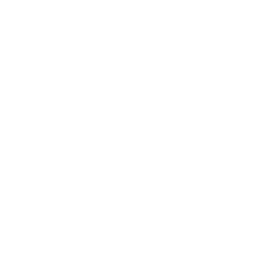
\includegraphics[scale=1]{assets/branding/opa0}
    \vspace{-5.75cm}\\
    {\adjustbox{scale=2.15}{\color{TealDarkCyan}\;III.\;Hamming Codes}}
    \bigskip\bigskip
    {\ }\vspace{4cm}\\
    \bigskip
  \end{center}
\end{frame}

\begin{frame}{\textbf{III. Hamming Codes}}{The design problem}
\small
\begin{block}{Goal}
Construct binary linear codes that correct exactly one error and use all possible syndromes.
\end{block}
\begin{itemize}
  \item A received word has either no error or one error in position $i$.
  \item Thus there are $1+n$ elementary cases.
  \item With $r$ parity checks, there are $2^r$ syndromes.
\end{itemize}
\[
  1+n=2^r
  \quad\Rightarrow\quad
  n=2^r-1.
\]
\end{frame}

\begin{frame}{\textbf{III. Hamming Codes}}{The parity-check matrix}
\small
\defbox[Binary Hamming matrix]{
For $r\ge2$, let $H_r$ be the $r\times(2^r-1)$ matrix whose columns are all nonzero vectors of $\F_2^r$.
}
\[
  H_3=
  \begin{bmatrix}
  1&0&1&0&1&0&1\\
  0&1&1&0&0&1&1\\
  0&0&0&1&1&1&1
  \end{bmatrix}.
\]
\begin{itemize}
  \item Column labels are nonzero binary syndromes.
  \item Every nonzero syndrome identifies a unique column.
\end{itemize}
\end{frame}

\begin{frame}{\textbf{III. Hamming Codes}}{Definition}
\small
\defbox[Binary Hamming code]{
The binary Hamming code of order $r$ is
\[
  \operatorname{Ham}(r,2)=\ker(H_r)\le\F_2^{2^r-1}.
\]
}
\begin{itemize}
  \item Length: $n=2^r-1$.
  \item Redundancy: $r$.
  \item Dimension: $k=n-r=2^r-1-r$.
\end{itemize}
\[
  \operatorname{Ham}(r,2)\text{ has parameters }[2^r-1,2^r-1-r,3]_2.
\]
\end{frame}

\begin{frame}{\textbf{III. Hamming Codes}}{Dimension}
\small
\thmbox[Dimension count]{
The matrix $H_r$ has rank $r$, hence
\[
  \dim\ker(H_r)=2^r-1-r.
\]
}
\begin{proof}
The standard basis vectors $e_1,\ldots,e_r$ occur among the nonzero columns of $H_r$, so the row rank is $r$.
\end{proof}
\begin{block}{Interpretation}
The parity checks are independent; no check is redundant.
\end{block}
\end{frame}

\begin{frame}{\textbf{III. Hamming Codes}}{Minimum distance}
\small
\thmbox[Distance]{
The binary Hamming code $\operatorname{Ham}(r,2)$ has minimum distance $3$.
}
\begin{proof}
No column of $H_r$ is zero, so $d\ge2$. No two columns are equal over $\F_2$, so no two are dependent, hence $d\ge3$. But $u+v+(u+v)=0$, so three suitable columns are dependent.
\end{proof}
\begin{itemize}
  \item Therefore Hamming codes correct one error.
  \item They detect two errors.
\end{itemize}
\end{frame}

\begin{frame}{\textbf{III. Hamming Codes}}{Perfectness}
\small
\thmbox[Hamming codes are perfect]{
The binary Hamming code satisfies equality in the Hamming bound for $t=1$.
}
\[
  2^k(1+n)=2^{2^r-1-r}(1+2^r-1)=2^{2^r-1}=2^n.
\]
\begin{itemize}
  \item Every word of $\F_2^n$ is at distance at most $1$ from exactly one codeword.
  \item The syndrome is not merely a diagnostic: it is a complete decoder.
\end{itemize}
\end{frame}

\begin{frame}{\textbf{III. Hamming Codes}}{Syndrome decoding}
\small
\defbox[Decoder]{
Given $v\in\F_2^n$, compute $s=H_rv^T$.
}
\begin{itemize}
  \item If $s=0$, accept $v$.
  \item If $s\ne0$, find the unique column $H_i=s$.
  \item Correct by flipping coordinate $i$.
\end{itemize}
\begin{block}{Reason}
For a single error $e_i$, the syndrome is $H_re_i^T=H_i$.
\end{block}
\end{frame}

\begin{frame}{\textbf{III. Hamming Codes}}{Binary index convention}
\small
\defbox[Indexed columns]{
If the $i$-th column of $H_r$ is the binary expansion of $i$, then the nonzero syndrome is literally the error position.
}
\[
  s=(1,0,1)^T\quad\leadsto\quad i=5
\]
depending on the chosen bit order.
\begin{itemize}
  \item This is a notational convention, not an invariant.
  \item It explains the classical parity-bit positions $1,2,4,\ldots$.
\end{itemize}
\end{frame}

\begin{frame}{\textbf{III. Hamming Codes}}{The classical [7,4,3] code}
\small
\[
H=
\begin{bmatrix}
1&0&1&0&1&0&1\\
0&1&1&0&0&1&1\\
0&0&0&1&1&1&1
\end{bmatrix}.
\]
\begin{itemize}
  \item There are $7$ nonzero syndromes.
  \item Each syndrome names one error coordinate.
  \item The kernel has dimension $4$.
\end{itemize}
\[
  \operatorname{Ham}(3,2)=[7,4,3]_2.
\]
\end{frame}

\begin{frame}{\textbf{III. Hamming Codes}}{A systematic generator matrix}
\small
One systematic form for the $[7,4,3]$ Hamming code is
\[
G=
\begin{bmatrix}
1&0&0&0&0&1&1\\
0&1&0&0&1&0&1\\
0&0&1&0&1&1&0\\
0&0&0&1&1&1&1
\end{bmatrix}.
\]
\begin{itemize}
  \item The first four coordinates are message symbols.
  \item The last three are parity symbols.
  \item This $G$ is equivalent to the kernel of a suitable $H$.
\end{itemize}
\end{frame}

\begin{frame}{\textbf{III. Hamming Codes}}{Encoding example}
\small
For $m=(1,0,1,1)$ and the systematic matrix $G$,
\[
  c=mG=(1,0,1,1,0,0,1).
\]
\begin{itemize}
  \item The parity bits are linear forms in the message bits.
  \item A single flipped bit changes the syndrome to the corresponding column.
  \item The correction rule does not require knowing the transmitted message.
\end{itemize}
\end{frame}

\begin{frame}{\textbf{III. Hamming Codes}}{Projective geometry}
\small
\defbox[Projective interpretation]{
The nonzero columns of $H_r$, modulo scalar multiplication, are the points of projective space
\[
  \mathbb{P}^{r-1}(\F_q).
\]
}
\begin{itemize}
  \item Over $\F_2$, each nonzero vector is its own projective point.
  \item Over $\F_q$, scalar multiples define the same projective point.
  \item Hamming codes are parity checks indexed by projective points.
\end{itemize}
\end{frame}

\begin{frame}{\textbf{III. Hamming Codes}}{The Fano plane}
\small
For $r=3$, the projective space $\mathbb{P}^2(\F_2)$ has $7$ points and $7$ lines.
\begin{itemize}
  \item The $7$ columns of $H_3$ are the points.
  \item A dependent triple of columns is a line of the Fano plane.
  \item Weight-$3$ codewords are exactly these lines.
\end{itemize}
\begin{block}{Geometry}
The minimum distance $3$ is the statement that the smallest projective line has three points.
\end{block}
\end{frame}

\begin{frame}{\textbf{III. Hamming Codes}}{Lines give codewords}
\small
In $\mathbb{P}^2(\F_2)$, if $a,b,c$ are the three points on a line, then
\[
  a+b+c=0.
\]
\begin{itemize}
  \item The incidence vector of that line is a Hamming codeword.
  \item The $7$ lines give the $7$ words of weight $3$.
  \item Their complements give $7$ words of weight $4$.
\end{itemize}
\[
  W_{\operatorname{Ham}(3,2)}(Y)=1+7Y^3+7Y^4+Y^7.
\]
\end{frame}

\begin{frame}{\textbf{III. Hamming Codes}}{The simplex dual}
\small
\defbox[Simplex code]{
The row space of $H_r$ is the binary simplex code:
\[
  \operatorname{Sim}(r,2)=\operatorname{rowspan}(H_r).
\]
}
\begin{itemize}
  \item It has parameters $[2^r-1,r,2^{r-1}]_2$.
  \item Every nonzero word has weight $2^{r-1}$.
  \item It is dual to the Hamming code.
\end{itemize}
\[
  \operatorname{Ham}(r,2)^\perp=\operatorname{Sim}(r,2).
\]
\end{frame}

\begin{frame}{\textbf{III. Hamming Codes}}{MacWilliams check}
\small
For $r=3$, the simplex code has weight enumerator
\[
  W_{\operatorname{Sim}}(X,Y)=X^7+7X^3Y^4.
\]
Applying MacWilliams gives
\[
  W_{\operatorname{Ham}}(X,Y)=X^7+7X^4Y^3+7X^3Y^4+Y^7.
\]
\begin{itemize}
  \item The algebraic transform recovers the geometric weight distribution.
  \item Duality is visible both in matrices and in enumerators.
\end{itemize}
\end{frame}

\begin{frame}{\textbf{III. Hamming Codes}}{Q-ary Hamming codes}
\small
\defbox[Q-ary construction]{
Choose one nonzero representative from each one-dimensional subspace of $\F_q^r$ and use these vectors as columns of $H$.
}
\[
  n=\frac{q^r-1}{q-1}.
\]
\begin{itemize}
  \item The resulting code has parameters
  \[
    \left[\frac{q^r-1}{q-1},\frac{q^r-1}{q-1}-r,3\right]_q.
  \]
  \item It is again perfect for one-error correction.
\end{itemize}
\end{frame}

\begin{frame}{\textbf{III. Hamming Codes}}{Why projective representatives}
\small
Over $\F_q$, two proportional nonzero columns are linearly dependent.
\begin{itemize}
  \item To have $d\ge3$, no two columns may be proportional.
  \item Therefore columns must be projective points, not raw nonzero vectors.
  \item Taking all projective points uses the maximum possible number of columns.
\end{itemize}
\begin{block}{Conclusion}
Hamming codes are the maximal parity-check configurations with no zero column and no repeated projective point.
\end{block}
\end{frame}

\begin{frame}{\textbf{III. Hamming Codes}}{Q-ary perfectness}
\small
For the $q$-ary Hamming code,
\[
  n=\frac{q^r-1}{q-1},\qquad k=n-r.
\]
The radius-one sphere has size
\[
  1+n(q-1)=1+q^r-1=q^r.
\]
Hence
\[
  q^k(1+n(q-1))=q^{n-r}q^r=q^n.
\]
\begin{block}{Perfect again}
Every received word lies at distance at most one from a unique codeword.
\end{block}
\end{frame}

\begin{frame}{\textbf{III. Hamming Codes}}{Extended Hamming codes}
\small
\defbox[Extension]{
Add one overall parity coordinate to force even total weight.
}
\begin{itemize}
  \item The binary $[7,4,3]$ code becomes an $[8,4,4]$ code.
  \item The new minimum distance is $4$.
  \item It detects three errors and corrects one error.
\end{itemize}
\[
  \widehat{\operatorname{Ham}}(3,2)=[8,4,4]_2.
\]
\end{frame}

\begin{frame}{\textbf{III. Hamming Codes}}{The [8,4,4] code}
\small
The extended Hamming code has weight enumerator
\[
  W(X,Y)=X^8+14X^4Y^4+Y^8.
\]
\begin{itemize}
  \item All codeword weights are divisible by $4$.
  \item The code is self-dual.
  \item It is the smallest doubly-even self-dual binary code.
\end{itemize}
\begin{block}{Connection}
This code is the length-$8$ seed behind the $E_8$ lattice construction.
\end{block}
\end{frame}

\begin{frame}{\textbf{III. Hamming Codes}}{Automorphisms}
\small
\defbox[Symmetry group]{
The automorphism group of the binary Hamming code is induced by invertible linear transformations of $\F_2^r$:
\[
  \Aut(\operatorname{Ham}(r,2))\cong \operatorname{GL}(r,2).
\]
}
\begin{itemize}
  \item A matrix in $\operatorname{GL}(r,2)$ permutes the nonzero columns of $H_r$.
  \item Hence it permutes coordinates and preserves the kernel.
  \item The code remembers the projective geometry.
\end{itemize}
\end{frame}

\begin{frame}{\textbf{III. Hamming Codes}}{Tanner graph}
\small
\begin{itemize}
  \item The Tanner graph of $H_r$ has $n=2^r-1$ variable nodes and $r$ check nodes.
  \item It is dense compared with modern LDPC codes.
  \item But it has an exceptionally simple exact decoder.
\end{itemize}
\begin{block}{Interpretation}
For Hamming codes, the syndrome is not iteratively refined; it is read directly as a projective point.
\end{block}
\end{frame}

\begin{frame}{\textbf{III. Hamming Codes}}{Failure modes}
\small
\begin{itemize}
  \item A two-error pattern has syndrome equal to the sum of two columns.
  \item In a binary Hamming matrix, that sum is another nonzero column.
  \item Therefore a two-error pattern may be miscorrected as a one-error pattern.
\end{itemize}
\begin{block}{Moral}
Minimum distance $3$ guarantees single-error correction, not reliable detection after attempting correction.
\end{block}
\end{frame}

\begin{frame}{\textbf{III. Hamming Codes}}{SECDED}
\small
\defbox[SECDED]{
Single-error correction, double-error detection is obtained by using the extended Hamming code.
}
\begin{itemize}
  \item The extension raises the distance from $3$ to $4$.
  \item One error is corrected by the Hamming syndrome.
  \item Two errors are detected because parity and syndrome disagree in a recognizable way.
\end{itemize}
\end{frame}

\begin{frame}{\textbf{III. Hamming Codes}}{Shortened Hamming codes}
\small
\defbox[Shortening]{
Shortened Hamming codes are obtained by fixing selected coordinates to zero and deleting them.
}
\begin{itemize}
  \item They are useful when exact lengths $2^r-1$ are inconvenient.
  \item The minimum distance remains at least $3$.
  \item Perfectness is usually lost.
\end{itemize}
\begin{block}{Engineering}
Many practical memory codes are shortened or extended Hamming codes.
\end{block}
\end{frame}

\begin{frame}{\textbf{III. Hamming Codes}}{Hamming codes as BCH codes}
\small
\defbox[Cyclic viewpoint]{
When $n=2^r-1$, the binary Hamming code can be realized as a narrow-sense BCH code of designed distance $3$.
}
\begin{itemize}
  \item Choose a primitive $n$-th root $\alpha\in\F_{2^r}$.
  \item Let $g(X)$ be the minimal polynomial of $\alpha$ over $\F_2$.
  \item Then the cyclic code generated by $g(X)$ is a Hamming code.
\end{itemize}
\end{frame}

\begin{frame}{\textbf{III. Hamming Codes}}{The [7,4,3] cyclic form}
\small
Over $\F_2$,
\[
  X^7-1=(X+1)(X^3+X+1)(X^3+X^2+1).
\]
Taking
\[
  g(X)=X^3+X+1
\]
gives a cyclic $[7,4,3]$ Hamming code.
\begin{itemize}
  \item This is the bridge from projective checks to polynomial ideals.
  \item The next chapter makes that bridge systematic.
\end{itemize}
\end{frame}

\begin{frame}{\textbf{III. Hamming Codes}}{Classification intuition}
\small
\begin{itemize}
  \item Perfect one-error-correcting linear codes are essentially Hamming codes, apart from trivial cases.
  \item The parity-check matrix must use every possible nonzero syndrome once.
  \item Thus the construction is forced by the Hamming bound.
\end{itemize}
\begin{block}{Mathematical taste}
Hamming codes are beautiful because optimality, decoding, and geometry are the same statement.
\end{block}
\end{frame}

\begin{frame}{\textbf{III. Hamming Codes}}{Exercise: distance}
\small
\begin{block}{Problem}
Let $H$ contain one representative of every point of $\mathbb{P}^{r-1}(\F_q)$. Prove that $\ker H$ has distance exactly $3$.
\end{block}
\textbf{Hint.}
\begin{itemize}
  \item No one or two columns are dependent.
  \item Any projective line contains three dependent representatives after scaling.
  \item Translate column dependence into a codeword support.
\end{itemize}
\end{frame}

\begin{frame}{\textbf{III. Hamming Codes}}{Exercise: perfectness}
\small
\begin{block}{Problem}
Verify directly that the $q$-ary Hamming code meets the Hamming bound with equality for $t=1$.
\end{block}
\[
  n=\frac{q^r-1}{q-1},\qquad k=n-r.
\]
\textbf{Computation.}
\[
  q^k(1+n(q-1))=q^{n-r}(1+q^r-1)=q^n.
\]
\end{frame}

\begin{frame}{\textbf{III. Hamming Codes}}{Exercise: dual weights}
\small
\begin{block}{Problem}
Show that every nonzero word of the binary simplex code has weight $2^{r-1}$.
\end{block}
\textbf{Hint.}
For a nonzero row vector $a\in\F_2^r$, the word $aH_r$ evaluates the nonzero linear functional $x\mapsto ax^T$ on every nonzero vector $x$.
\begin{itemize}
  \item Exactly half of all vectors of $\F_2^r$ evaluate to $1$.
  \item The zero vector evaluates to $0$.
\end{itemize}
\end{frame}

\begin{frame}{\textbf{III. Hamming Codes}}{Summary}
\small
\begin{columns}[T,onlytextwidth]
  \begin{column}{.48\textwidth}
    \defbox[Construction]{
    \begin{itemize}\small
      \item parity-check columns are projective points
      \item no repeated projective column
      \item all syndromes are used
    \end{itemize}
    }
  \end{column}
  \begin{column}{.48\textwidth}
    \defbox[Consequences]{
    \begin{itemize}\small
      \item parameters $[2^r-1,2^r-1-r,3]_2$
      \item perfect one-error correction
      \item dual simplex code
    \end{itemize}
    }
  \end{column}
\end{columns}
\end{frame}

\begin{frame}{\textbf{III. Hamming Codes}}{Transition to cyclic codes}
\small
\begin{block}{New symmetry}
Hamming codes are governed by projective geometry. Cyclic codes are governed by the cyclic shift operator.
\end{block}
\begin{itemize}
  \item Linear code: subspace of $\F_q^n$.
  \item Hamming code: subspace defined by projective parity checks.
  \item Cyclic code: subspace stable under a cyclic permutation.
\end{itemize}
\[
  \text{shift symmetry}\quad\Longleftrightarrow\quad\text{ideals in }\F_q[X]/(X^n-1).
\]
\end{frame}



%-------------------------------------------------------
% IV. CYCLIC CODES
%-------------------------------------------------------
\section{IV. Cyclic Codes}
%=======================================================
% CHAPTER 3: CYCLIC CODES
%=======================================================

\begin{frame}[plain]
  \begin{center}\bfseries\centering
    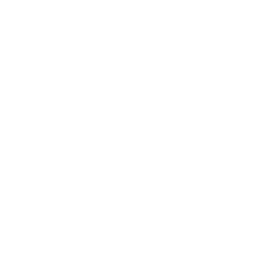
\includegraphics[scale=1]{assets/branding/opa0}
    \vspace{-5.75cm}\\
    {\adjustbox{scale=2.15}{\color{TealDarkCyan}\;IV.\;Cyclic Codes}}
    \bigskip\bigskip
    {\ }\vspace{4cm}\\
    \bigskip
  \end{center}
\end{frame}

\begin{frame}{\textbf{IV. Cyclic Codes}}{Cyclic shift}
\small
\defbox[Cyclic code]{
A linear code $\code\le\F_q^n$ is cyclic if
\[
  (c_0,c_1,\ldots,c_{n-1})\in\code
  \quad\Rightarrow\quad
  (c_{n-1},c_0,\ldots,c_{n-2})\in\code.
\]
}
\begin{itemize}
  \item This is invariance under a single permutation.
  \item Since the permutation has order $n$, cyclic codes are modules over a cyclic group algebra.
  \item The polynomial model makes this precise.
\end{itemize}
\end{frame}

\begin{frame}{\textbf{IV. Cyclic Codes}}{Polynomial dictionary}
\small
\defbox[Vector to polynomial]{
Identify
\[
  (c_0,c_1,\ldots,c_{n-1})
  \quad\longleftrightarrow\quad
  c(X)=c_0+c_1X+\cdots+c_{n-1}X^{n-1}.
\]
}
\begin{itemize}
  \item Multiplication by $X$ shifts coefficients.
  \item The relation $X^n=1$ performs wrap-around.
  \item Therefore we work modulo $X^n-1$.
\end{itemize}
\end{frame}

\begin{frame}{\textbf{IV. Cyclic Codes}}{The quotient ring}
\small
\defbox[Ambient ring]{
\[
  R_n=\F_q[X]/(X^n-1).
\]
}
\begin{itemize}
  \item Vectors of length $n$ are polynomials of degree $<n$.
  \item Cyclic shift is multiplication by $X$ in $R_n$.
  \item A cyclic code is an $\F_q$-subspace stable under multiplication by $X$.
\end{itemize}
\begin{block}{Key question}
Which subspaces of $R_n$ are stable under multiplication by $X$?
\end{block}
\end{frame}

\begin{frame}{\textbf{IV. Cyclic Codes}}{Ideals}
\small
\thmbox[Cyclic codes are ideals]{
Under the identification $\F_q^n\cong R_n$, cyclic codes are exactly the ideals of $R_n$.
}
\begin{proof}
If $\code$ is stable under multiplication by $X$, then it is stable under multiplication by every polynomial in $X$. Hence it is an ideal. The converse is immediate.
\end{proof}
\begin{block}{Consequence}
The classification of cyclic codes is an ideal-theoretic problem.
\end{block}
\end{frame}

\begin{frame}{\textbf{IV. Cyclic Codes}}{Principal ideals}
\small
\thmbox[Principal generator]{
Every ideal of $R_n$ is generated by a unique monic divisor $g(X)$ of $X^n-1$:
\[
  \code=(g(X)).
\]
}
\begin{itemize}
  \item This follows from the principal ideal property of $\F_q[X]$.
  \item The generator polynomial is the monic element of least degree in the code.
  \item The divisibility condition is $g(X)\mid X^n-1$.
\end{itemize}
\end{frame}

\begin{frame}{\textbf{IV. Cyclic Codes}}{Dimension}
\small
\thmbox[Dimension formula]{
If $\code=(g(X))\subseteq R_n$ and $\deg g=r$, then
\[
  \dim_{\F_q}\code=n-r.
\]
}
\begin{proof}
The polynomials
\[
  g(X),Xg(X),\ldots,X^{n-r-1}g(X)
\]
form an $\F_q$-basis of the ideal.
\end{proof}
\end{frame}

\begin{frame}{\textbf{IV. Cyclic Codes}}{Generator matrix from shifts}
\small
If
\[
  g(X)=g_0+g_1X+\cdots+g_rX^r,
\]
then a generator matrix is obtained by shifting the coefficient vector:
\[
\begin{bmatrix}
g_0&g_1&\cdots&g_r&0&\cdots&0\\
0&g_0&g_1&\cdots&g_r&\cdots&0\\
\vdots&&\ddots&&&\ddots&\vdots
\end{bmatrix}.
\]
\begin{itemize}
  \item This matrix is Toeplitz-like.
  \item It encodes multiplication by $g(X)$.
\end{itemize}
\end{frame}

\begin{frame}{\textbf{IV. Cyclic Codes}}{Parity-check polynomial}
\small
\defbox[Check polynomial]{
If $g(X)\mid X^n-1$, define
\[
  h(X)=\frac{X^n-1}{g(X)}.
\]
}
\begin{itemize}
  \item $\deg h=k$ when $\code$ has dimension $k$.
  \item Since $g(X)h(X)=0$ in $R_n$, multiplication by $h(X)$ checks membership.
  \item More precisely, $c(X)\in(g)$ implies $c(X)h(X)\equiv0\pmod{X^n-1}$.
\end{itemize}
\end{frame}

\begin{frame}{\textbf{IV. Cyclic Codes}}{Reciprocal polynomials}
\small
\defbox[Reciprocal]{
For $f(X)=f_0+\cdots+f_mX^m$ with $f_0\ne0$, define
\[
  f^*(X)=X^mf(X^{-1}).
\]
}
\begin{itemize}
  \item Parity-check matrices are naturally written using reciprocal polynomials.
  \item The dual of a cyclic code is cyclic.
  \item If $\code=(g)$ and $h=(X^n-1)/g$, then $\code^\perp$ is generated by a reciprocal of $h$.
\end{itemize}
\end{frame}

\begin{frame}{\textbf{IV. Cyclic Codes}}{Idempotents}
\small
\defbox[Idempotent generator]{
When $\gcd(n,q)=1$, each cyclic code has a unique idempotent generator $e(X)$ satisfying
\[
  e(X)^2=e(X),\qquad \code=(e(X)).
\]
}
\begin{itemize}
  \item Idempotents decompose the semisimple ring $R_n$.
  \item They expose the representation-theoretic structure.
  \item Generator polynomials are usually better for computation.
\end{itemize}
\end{frame}

\begin{frame}{\textbf{IV. Cyclic Codes}}{Roots}
\small
Let $\alpha$ be an $n$-th root of unity in an extension field.
\begin{itemize}
  \item A cyclic code generated by $g(X)$ has zeros $\alpha^i$ where $g(\alpha^i)=0$.
  \item The defining set is
  \[
    Z(\code)=\{i\pmod n:g(\alpha^i)=0\}.
  \]
  \item Root sets translate algebraic divisibility into combinatorics modulo $n$.
\end{itemize}
\end{frame}

\begin{frame}{\textbf{IV. Cyclic Codes}}{Cyclotomic cosets}
\small
\defbox[Q-cyclotomic coset]{
Modulo $n$, the $q$-cyclotomic coset of $i$ is
\[
  C_i=\{i,iq,iq^2,\ldots\}\pmod n.
\]
}
\begin{itemize}
  \item If $\alpha^i$ is a root over $\F_q$, all conjugates $\alpha^{iq^j}$ are roots.
  \item Therefore defining sets are unions of cyclotomic cosets.
  \item Minimal polynomials correspond to these cosets.
\end{itemize}
\end{frame}

\begin{frame}{\textbf{IV. Cyclic Codes}}{Minimal polynomials}
\small
\defbox[Minimal polynomial]{
For $\alpha^i$, the minimal polynomial over $\F_q$ is
\[
  M_i(X)=\prod_{j\in C_i}(X-\alpha^j).
\]
}
\begin{itemize}
  \item It lies in $\F_q[X]$.
  \item It is irreducible.
  \item Generator polynomials of cyclic codes are products of such $M_i(X)$.
\end{itemize}
\end{frame}

\begin{frame}{\textbf{IV. Cyclic Codes}}{BCH codes}
\small
\defbox[BCH design]{
A BCH code is a cyclic code whose generator polynomial has a prescribed block of consecutive roots.
}
\[
  g(\alpha^b)=g(\alpha^{b+1})=\cdots=g(\alpha^{b+\delta-2})=0.
\]
\begin{itemize}
  \item The integer $\delta$ is the designed distance.
  \item Consecutive roots force many syndromes to vanish.
  \item The BCH bound converts this into a distance guarantee.
\end{itemize}
\end{frame}

\begin{frame}{\textbf{IV. Cyclic Codes}}{BCH bound}
\small
\thmbox[BCH bound]{
If a cyclic code has $\delta-1$ consecutive roots
\[
  \alpha^b,\alpha^{b+1},\ldots,\alpha^{b+\delta-2},
\]
then its minimum distance is at least $\delta$.
}
\begin{proof}
A codeword of weight $<\delta$ would give a nonzero polynomial with too many consecutive zero syndromes, forcing a Vandermonde determinant to vanish.
\end{proof}
\end{frame}

\begin{frame}{\textbf{IV. Cyclic Codes}}{Narrow-sense primitive BCH}
\small
\defbox[Common special case]{
Let $n=q^m-1$ and let $\alpha$ be primitive in $\F_{q^m}$. The narrow-sense BCH code of designed distance $\delta$ has roots
\[
  \alpha,\alpha^2,\ldots,\alpha^{\delta-1}.
\]
}
\begin{itemize}
  \item Primitive: the length is the full multiplicative order.
  \item Narrow-sense: the first root is $\alpha$.
  \item Hamming codes occur when $\delta=3$ in the binary case.
\end{itemize}
\end{frame}

\begin{frame}{\textbf{IV. Cyclic Codes}}{Cyclic Hamming code}
\small
Let $n=2^r-1$ and let $\alpha\in\F_{2^r}$ be primitive.
\begin{itemize}
  \item Let $g(X)$ be the minimal polynomial of $\alpha$ over $\F_2$.
  \item Then $\deg g=r$.
  \item The cyclic code $(g)$ has parameters
  \[
    [2^r-1,2^r-1-r,3]_2.
  \]
\end{itemize}
\begin{block}{Identification}
This is the binary Hamming code in cyclic coordinates.
\end{block}
\end{frame}

\begin{frame}{\textbf{IV. Cyclic Codes}}{The case n equals 7}
\small
Over $\F_2$,
\[
  X^7-1=(X+1)(X^3+X+1)(X^3+X^2+1).
\]
\begin{itemize}
  \item A primitive $7$-th root has minimal polynomial $X^3+X+1$ or $X^3+X^2+1$.
  \item Either cubic gives a cyclic $[7,4,3]$ Hamming code.
  \item The two choices are equivalent under coordinate reversal.
\end{itemize}
\end{frame}

\begin{frame}{\textbf{IV. Cyclic Codes}}{Encoding by multiplication}
\small
For a cyclic code $(g)$ with $\deg g=r$, non-systematic encoding is
\[
  m(X)\longmapsto c(X)=m(X)g(X),\qquad \deg m< n-r.
\]
\begin{itemize}
  \item The message polynomial has $k=n-r$ coefficients.
  \item The product automatically lies in the ideal $(g)$.
  \item Hardware can implement this multiplication by shift registers.
\end{itemize}
\end{frame}

\begin{frame}{\textbf{IV. Cyclic Codes}}{Systematic cyclic encoding}
\small
Let $\deg g=r$. To encode a message $m(X)$ with $\deg m<k$:
\[
  X^r m(X)=q(X)g(X)+p(X),\qquad \deg p<r.
\]
Then set
\[
  c(X)=X^rm(X)-p(X).
\]
\begin{itemize}
  \item Since $c(X)$ is divisible by $g(X)$, it is a codeword.
  \item The high-degree coefficients contain the message.
  \item The low-degree polynomial $p(X)$ supplies parity.
\end{itemize}
\end{frame}

\begin{frame}{\textbf{IV. Cyclic Codes}}{Syndrome polynomial}
\small
For received $v(X)=c(X)+e(X)$, compute the remainder
\[
  s(X)=v(X)\bmod g(X).
\]
\begin{itemize}
  \item Since $c(X)$ is divisible by $g(X)$, $s(X)=e(X)\bmod g(X)$.
  \item This is the polynomial analogue of $Hv^T=He^T$.
  \item BCH decoding refines this by evaluating at roots of $g$.
\end{itemize}
\end{frame}

\begin{frame}{\textbf{IV. Cyclic Codes}}{Root syndromes}
\small
If $\alpha^i$ is a root of $g(X)$, then every codeword satisfies
\[
  c(\alpha^i)=0.
\]
For $v=c+e$,
\[
  v(\alpha^i)=e(\alpha^i).
\]
\begin{itemize}
  \item The numbers $S_i=v(\alpha^i)$ are syndromes.
  \item Decoding asks for the error locations and values from these sums.
  \item This is a finite-field moment problem.
\end{itemize}
\end{frame}

\begin{frame}{\textbf{IV. Cyclic Codes}}{Error locator polynomial}
\small
For error locations $j_1,\ldots,j_t$, define
\[
  \Lambda(Z)=\prod_{\ell=1}^t(1-\alpha^{j_\ell}Z).
\]
\begin{itemize}
  \item The roots of $\Lambda$ identify error locations.
  \item BCH and Reed--Solomon decoding compute $\Lambda$ from syndromes.
  \item Berlekamp--Massey is an efficient algorithm for this recurrence problem.
\end{itemize}
\end{frame}

\begin{frame}{\textbf{IV. Cyclic Codes}}{LFSR viewpoint}
\small
\defbox[Linear feedback shift register]{
Division by $g(X)$ can be implemented with a shift register whose feedback taps are the nonzero coefficients of $g(X)$.
}
\begin{itemize}
  \item Memory cost is $\deg g=n-k$ registers.
  \item Input is processed one symbol per clock.
  \item This is why cyclic codes became central in hardware error control.
\end{itemize}
\end{frame}

\begin{frame}{\textbf{IV. Cyclic Codes}}{Burst errors}
\small
\defbox[Burst]{
A burst of length $\ell$ is an error whose nonzero positions lie in $\ell$ consecutive coordinates.
}
\begin{itemize}
  \item Polynomial remainders are well suited for burst detection.
  \item CRC polynomials are chosen to detect common burst patterns.
  \item This is detection rather than correction in many communication protocols.
\end{itemize}
\end{frame}

\begin{frame}{\textbf{IV. Cyclic Codes}}{CRC codes}
\small
CRC uses a generator polynomial $g(X)$ and transmits a multiple of $g(X)$.
\begin{itemize}
  \item Receiver divides by $g(X)$.
  \item Nonzero remainder means an error was detected.
  \item The method is a cyclic-code membership test.
\end{itemize}
\begin{block}{Mathematical core}
CRC is not a different theory: it is cyclic codes used primarily for error detection.
\end{block}
\end{frame}

\begin{frame}{\textbf{IV. Cyclic Codes}}{Reed--Solomon codes}
\small
\defbox[Reed--Solomon]{
Over $\F_q$, Reed--Solomon codes evaluate polynomials of degree $<k$ at $n$ distinct field points.
}
\begin{itemize}
  \item In a suitable form, they are cyclic codes.
  \item They meet the Singleton bound: $d=n-k+1$.
  \item They correct symbol errors, which is why they are strong against bursts.
\end{itemize}
\end{frame}

\begin{frame}{\textbf{IV. Cyclic Codes}}{BCH versus Reed--Solomon}
\small
\begin{columns}[T,onlytextwidth]
  \begin{column}{.48\textwidth}
    \defbox[BCH]{
    \begin{itemize}\small
      \item often binary
      \item roots in an extension field
      \item designed distance
      \item strong for bit errors
    \end{itemize}
    }
  \end{column}
  \begin{column}{.48\textwidth}
    \defbox[Reed--Solomon]{
    \begin{itemize}\small
      \item nonbinary
      \item evaluation over $\F_q$
      \item MDS property
      \item strong for symbol bursts
    \end{itemize}
    }
  \end{column}
\end{columns}
\end{frame}

\begin{frame}{\textbf{IV. Cyclic Codes}}{Dual cyclic codes}
\small
\thmbox[Dual cyclicity]{
The dual of a cyclic code is cyclic.
}
\begin{proof}
If $c$ is orthogonal to every word of $\code$, then a cyclic shift of $c$ is also orthogonal to every cyclic shift of every word of $\code$. Since $\code$ is shift-invariant, the shifted $c$ lies in $\code^\perp$.
\end{proof}
\begin{itemize}
  \item Generator polynomials of duals are expressed using reciprocal polynomials.
  \item This is another sign that cyclic codes form a closed algebraic world.
\end{itemize}
\end{frame}

\begin{frame}{\textbf{IV. Cyclic Codes}}{Repeated-root caution}
\small
\begin{block}{Assumption often made}
Many clean statements assume $\gcd(n,q)=1$.
\end{block}
\begin{itemize}
  \item Then $X^n-1$ has no repeated roots.
  \item The quotient ring is semisimple.
  \item If $\gcd(n,q)\ne1$, repeated-root cyclic codes require extra care.
\end{itemize}
\begin{block}{Moral}
Always check separability before using root-set arguments naively.
\end{block}
\end{frame}

\begin{frame}{\textbf{IV. Cyclic Codes}}{Quasi-cyclic hint}
\small
\defbox[Quasi-cyclic code]{
A code is quasi-cyclic of index $\ell$ if it is invariant under cyclic shift by $\ell$ positions.
}
\begin{itemize}
  \item Generator matrices are built from circulant blocks.
  \item Circulant blocks correspond to polynomials modulo $X^m-1$.
  \item This structure is important in code-based cryptography.
\end{itemize}
\end{frame}

\begin{frame}{\textbf{IV. Cyclic Codes}}{Algebraic hierarchy}
\small
\[
\begin{array}{c}
\text{linear code}\\
\Downarrow\ \text{add cyclic shift}\\
\text{cyclic code}\\
\Downarrow\ \text{prescribe roots}\\
\text{BCH code}\\
\Downarrow\ \text{evaluation/MDS structure}\\
\text{Reed--Solomon code}
\end{array}
\]
\begin{block}{Perspective}
Each additional algebraic structure buys stronger theorems and faster algorithms.
\end{block}
\end{frame}

\begin{frame}{\textbf{IV. Cyclic Codes}}{Cyclic codes as modules}
\small
\begin{itemize}
  \item A linear code is an $\F_q$-subspace of $\F_q^n$.
  \item A cyclic code is an $\F_q[X]$-submodule, where $X$ acts by shift.
  \item The relation $X^n=1$ makes the module a module over $R_n$.
\end{itemize}
\[
  \text{cyclic code}=\text{submodule of }R_n=\text{ideal of }R_n.
\]
\begin{block}{Mathematician's slogan}
Shift-invariant linear algebra is ideal theory.
\end{block}
\end{frame}

\begin{frame}{\textbf{IV. Cyclic Codes}}{Exercise: ideal proof}
\small
\begin{block}{Problem}
Prove that if an $\F_q$-subspace $\code\subseteq R_n$ is closed under multiplication by $X$, then it is an ideal.
\end{block}
\textbf{Hint.}
\begin{itemize}
  \item Closure under $X$ gives closure under $X^j$ for every $j\ge0$.
  \item By linearity, closure under every polynomial follows.
  \item Reduce modulo $X^n-1$.
\end{itemize}
\end{frame}

\begin{frame}{\textbf{IV. Cyclic Codes}}{Exercise: dimension}
\small
\begin{block}{Problem}
Let $g(X)\mid X^n-1$ and $\deg g=r$. Show that $(g)$ has dimension $n-r$ as an $\F_q$-space.
\end{block}
\textbf{Hint.}
\[
  a(X)g(X),\qquad \deg a<n-r
\]
are all distinct modulo $X^n-1$.
\begin{itemize}
  \item Count the possible coefficients of $a(X)$.
  \item Use the degree bound to prove injectivity.
\end{itemize}
\end{frame}

\begin{frame}{\textbf{IV. Cyclic Codes}}{Exercise: cyclic Hamming}
\small
\begin{block}{Problem}
For $X^7-1=(X+1)(X^3+X+1)(X^3+X^2+1)$ over $\F_2$, show that the code generated by $g=X^3+X+1$ has parameters $[7,4,3]$.
\end{block}
\textbf{Hint.}
\begin{itemize}
  \item Dimension is $7-\deg g=4$.
  \item The BCH bound with roots $\alpha,\alpha^2$ gives $d\ge3$.
  \item The Singleton bound excludes $d>4$, and a direct word gives $d=3$.
\end{itemize}
\end{frame}

\begin{frame}{\textbf{IV. Cyclic Codes}}{Summary of cyclic codes}
\small
\begin{columns}[T,onlytextwidth]
  \begin{column}{.48\textwidth}
    \defbox[Algebra]{
    \begin{itemize}\small
      \item $R_n=\F_q[X]/(X^n-1)$
      \item cyclic codes are ideals
      \item generator polynomial $g$
      \item root sets and cosets
    \end{itemize}
    }
  \end{column}
  \begin{column}{.48\textwidth}
    \defbox[Algorithms]{
    \begin{itemize}\small
      \item encoding by multiplication
      \item parity by remainders
      \item BCH decoding from syndromes
      \item LFSR implementation
    \end{itemize}
    }
  \end{column}
\end{columns}
\end{frame}

\begin{frame}{\textbf{IV. Cyclic Codes}}{Final perspective}
\small
\begin{alertblock}{}
\centering
Linear codes turn error correction into finite-dimensional algebra.\\[4pt]
Hamming codes show how perfect decoding is finite geometry.\\[4pt]
Cyclic codes show how shift symmetry becomes polynomial ideal theory.
\end{alertblock}
\bigskip
\begin{center}
\large
\textbf{Coding theory is the art of adding structure to redundancy.}
\end{center}
\end{frame}


%-------------------------------------------------------
% CLOSING FRAME
%-------------------------------------------------------
%\begin{frame}[plain]
%  \begin{center}\bfseries\centering
%%    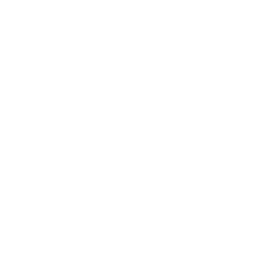
\includegraphics[scale=1]{assets/branding/opa0}
%%    \vspace{-6cm}\\
%    {\Huge\color{TealDarkCyan} Thank You}\\[.5cm]
%    {\large\color{black} Ji, Yong-hyeon}\\[.3cm]
%    {\normalsize\texttt{hacker3740@gmail.com}}\\[.5cm]
%    {\small\color{gray} 수학의 즐거움 $\cdot$ Enjoying Math $\cdot$ 2026}
%    \bigskip
%  \end{center}
%\end{frame}

\end{document}
